\section{System Design} % talk about general blackboard system structure

A Blackboard System is a way for distinct agents specializing in subproblems to communicate partial solutions and cooperate to find a complete solution.
There are three components of a Blackboard System: the Blackboard, the Control, and the Knowledge Sources.
Knowledge Sources are the specialized agents. They examine the Blackboard as input and write their partial solutions on the Blackboard.
The Blackboard is a data structure shared by all the Knowledge Sources and presided over by the Control. It is essentially an open read and write area.
The Control decides which Knowledge Sources run and when the problem has been solved.

\begin{figure}[h]
\centering
	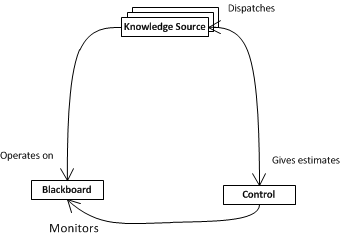
\includegraphics[keepaspectratio=true]{blackboard-system-diagram.png}
\caption{Structure of a general blackboard system}
\end{figure}

\subsection{Blackboard} % talk about the specific blackboard used

For this music composition system, the Blackboard contains two major items: the given musical line, the \emph{cantus firmus}, and the musical line in the progress of composition, the \emph{counterpoint}.
Both the \emph{cantus firmus} and the counterpoint are Voices (see appendix), but the \emph{cantus firmus} is read-only.
%Both provide a context-aware location reference (known as a Zipper) that makes it easier for Knowledge Sources and the Control to communicate about particular areas of a composition.
The Blackboard also contains other minor, but important, information such as the key or mode of the composition. This is mainly for ease of reference.
% TODO move this part into the discussion of the Control
%An important aspect of our implementation is that the Blackboard is immutable, a side effect of using Haskell as the implementation language.
%This is actually very useful because if a potential composition runs into a dead end, previous versions of the Blackboard are still around, making backtracking trivial.

\subsection{Knowledge Sources} % talk about the general structure for agents

Knowledge Sources, or agents, embody musical rules or preferences and can range from simple to complex.
Most of Counterpoint is specified by either forbidding certain kinds of musical structures or limiting their use so that others are preferred.
These are respectively known as `hard' and `soft' rules. Ideally, the system should not violate any hard rules and minimize violations of soft rules.
Agents embodying these rules essentially examine a location in a musical line and test whether their rule is upheld or not.
These agents exist to cut off the composition when it progresses in an undesirable way.

The counterpart to these tester agents are generators that modify the composition by extending it or changing an existing portion.
The most basic version of this type of agent just attaches random notes, within the allowed range, to the end of the existing composition.
More complex agents could make sweeping modifications to achieve higher level musical constructs.
For example, an agent could identify regions that are too flat (not enough vertical motion) and make them more contoured.

\subsection{Control} % talk about the control structure

The Control tracks the history of the Blackboard to help it choose how to precede.
The Control keeps a map from Blackboards to useful metadata: 
  which tests still need to run on that Blackboard,
  the parent Blackboard that this Blackboard was generated from,
  and the number and type of rule violations of this Blackboard and its descendents in vector form.
The Control picks the best Blackboard to operate on 
  where the best Blackboard has the minimal vector of violations under a lexicographic ordering 
  with ties broken by prefering Blackboards with longer counterpoints.
This ordering of Blackboards allows arbitrary backtracking and efficient comparison.

Using this record keeping scheme, the Control works as follows.
Get the best Blackboard $B$.
If the counterpoint of $B$ is as long as the \emph{cantus firmus} and $B$ has no queued tests, then the composition is complete.
If the counterpoint of $B$ is not long enough and $B$ has queued tests, run all those tests and record the results in the metadata. 
  Cascade changes in the violation vector up the chain of parents.
If the counterpoint of $B$ is not long enough and $B$ has no queued tests, pick a generator at random and apply it to $B$ to create $B'$.
  Identify which parts of the counterpoint changed in $B'$ relative to $B$ and queue tests for $B'$ to check those parts.
Identify the new best Blackboard and repeat.
